\subsection{Setting}

All evaluations were executed singled-threaded on an Intel Core i7-6700 CPU
running at 3.40GHz.

\paragraph{Input}
Here we explain the used reference graphs, reads, and error costs.

We designed three experiments utilizing three different reference graphs (in
\cref{TRIEtab:results}). The first is a linear graph without variation based on the
\textit{E.~coli} reference genome (strain: K-12 substr. MG1655,
ASM584v2~\cite{howe2019ensembl}). The other two are variation graphs taken from
the \pasgal evaluations~\cite{jain_accelerating_2019}: they are based on the
Leukocyte Receptor Complex (LRC, with \numprint{1099856} nodes and
\numprint{1144498} edges), and the Major Histocompatibility Complex (MHC1, with
\numprint{5138362} nodes and \numprint{5318019} edges).
%
We note that we do not evaluate on de Brujin graphs, since \pasgal does not
support cyclic graphs.

%\paragraph{Reads}
For the \textit{E.~coli} dataset we used the ART tool~\cite{huang_art_2012} to simulate an
Illumina single-end read set with \numprint{10000} reads of length 100. For the LCR and
MHC1 datasets, we sampled \numprint{20000} single-end reads of length 100 from the already
generated sets in~\cite{jain_accelerating_2019} using the
Mason2~\cite{holtgrewe_mason_2010} simulator.

We use costs corresponding to Illumina error profiles: $\Delta=(0,1,5,5)$.
%We apply all described optimizations.
% to, except
%\cref{TRIEsubsec:speedup-heuristic,TRIEsubsec:partition} which are applicable
%only to \astarix.

\paragraph{Metrics}
As all aligners evaluated here are provably optimal, we are mostly interested in
their performance.
%
To study the end-to-end performance of the optimal aligners, we use the
Snakemake~\cite{koster_snakemakescalable_2012} pipeline framework to measure the
execution time of every aligner (including the time spent on reading and
indexing the reference graph input and outputting the resulting alignments). We
note that the alignment phase dominates for all tools and experiments.

To judge the potential of heuristic functions, we measure not only the runtime
but also the number of states explored by \astarix and \dijkstra. This number
reflects the quality of the heuristic function rather than the speed of
computation of the heuristic, the implementation and the system parameters.
%"Fig. 3" (it also discusses explored states)}.
%The number of explored states is a more direct indicator for the algorithm's performance
%than the number of expanded states since the algorithm has to generate and consider
%all the neighbors of the states it expands.
%\todo{Harun: this argument only really works
%if computation of the heuristic is not a bottleneck. maybe make that more clear?}

\paragraph{Comparison to optimal aligners}

% Even though there is a variety of short read-to-graph aligners, only a few are
% guaranteed to be optimal.
We compare the performance of \astarix to that of two state-of-the-art optimal
aligners: \pasgal and \bitparallel, with their default parameters.
%
We do not compare to the exact aligner of \vg as (i)~its optimal alignment
is intended for testing purposes only, (ii)~it does not provide an
interface for aligning a set of reads, and (iii)~it has been consistently
outperformed by \pasgal~\cite{jain_accelerating_2019}.

\pasgal is compiled with AVX2 SIMD support. The resulting alignments are not
expected to match exactly between the local aligner \pasgal and the semi-global
aligners (\astarix and \bitparallel) as they solve different tasks with
different edit costs. Nevertheless, in analogy with the evaluations of
\pasgal~\cite{jain_accelerating_2019}, it is still meaningful to compare
performance, assuming that the dynamic programming approach of \pasgal can be
adapted to semi-global alignment with similar performance.

Both \bitparallel and \pasgal reach their worst-case runtime complexity
independent of the edit costs $\Delta=(\cmatch,\csubst,\cins,\cdel)$. \pasgal is
evaluated using its default costs ~$\Delta=(-1,1,1,1)$ and \bitparallel is
evaluated using the only supported costs~$\Delta=(0,1,1,1)$.

\paragraph{Parameter tuning} \label{TRIEsubsec:parameter_estimation}

While the optimality of \astarix is not affected by its parameters, its
performance is. To compare with other aligners, we use values \mbox{$d=5$},
\mbox{$\costcap=5$}, \mbox{$D = \lfloor \log_\Sigma \lvert \RG \rvert \rfloor$}.
Follows an investigation of the influence of different parameters ($\costcap$,
$d$, $D$) on the runtime and memory usage.

\begin{figure}[t]
	\centering
	\begin{minipage}{0.45\linewidth}
		\centering
		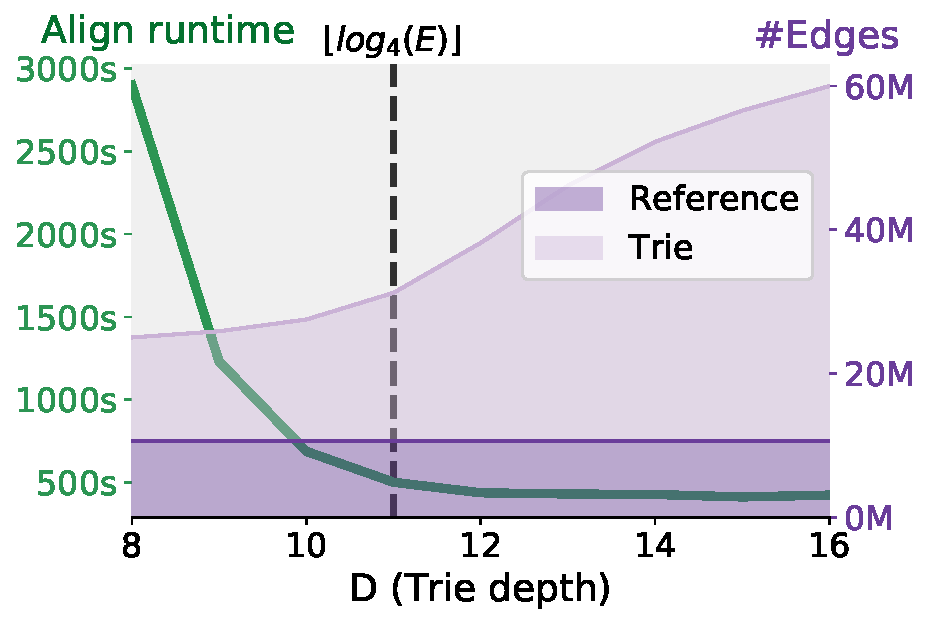
\includegraphics[width=\linewidth]{figs/trie/MHC1-trie-vs-D.pdf}
		\caption[Performance for various trie depths and heuristic parameters]{Left: Effect of the trie depth $D$ on the performance of \astarix (MHC1 experiment). The dashed line shows our choice of $D$. Right: Runtime of \astarix depending on $d$ and $\costcap$ (MHC1 experiment).}
		%\label{TRIEsubfig:MHC1-trie_vs_D}
		\label{TRIEfig:trie_vs_D}
	\end{minipage}%~\hspace{0.7em}
	\begin{minipage}{0.45\linewidth}
		\centering
		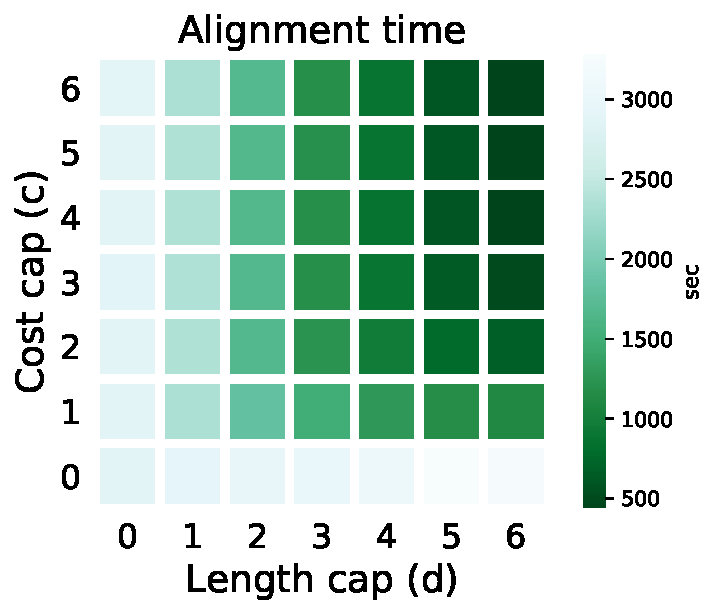
\includegraphics[width=0.8\linewidth]{figs/heuristic/MHC1-heatmap-c_vs_d-align_sec.pdf}
		%\caption{Runtime of \astarix depending on $d$ and $\costcap$ (MHC1 experiment).}
		\label{TRIEfig:heuristic-parameters}
	\end{minipage}
\end{figure}

\cref{TRIEfig:trie_vs_D} demonstrates the benefit of using a trie with the size
reduction optimization (end of \cref{TRIEsubsec:trie}): increasing the trie depth
$D$ speeds up aligning but requires more memory. Selecting the trie depth based
on the graph size \mbox{$D = \lfloor \log_\Sigma \lvert \RG \rvert \rfloor$}
provides a reasonable trade-off between alignment time and memory.

\cref{TRIEfig:heuristic-parameters} shows the joint effect of $\costcap$ and $d$. It
demonstrates that having a long reach ($d$) that covers at least some errors
($\costcap > 0$) is a reasonable strategy for choosing $d$ and $\costcap$.
